\section{Variational Autoencoder}
\label{sec:VAE}
A \ac{VAE} is an artificial neural network architecture itroduced by Diederik P. Kingma and Max Welling in 2013 \cite{originalVAEarticle}. These types of models connect an encoder neural network to its decoder counterpart through a probabilistic latent space, for instance Gaussian distributions. This means that the encoder maps each input point, i.e. a time series (waveform) in our case, into a distribution within the latent space, differently from the standard autoencoders where input points are mapped into a single point in the latent space. From said distributions, the decoder part reconsruct the time series. 
\subsection{Architecture}
\label{sec:vae-architeture}
\begin{comment}
QUI DEVO DIRE

-COME CREO I TENSORS --> TENSORCREATION.PY

-COME IMPLEMENTO IL VAE

    - encoder\\
    - decoder\\
    - latent space specifications\\
    - costruzione della loss\\
    - training\\ 
    - test\\
    - tutti i test del codice che faccio\\
        * test su beta
        * test su dimensioni dello spazio lentamente
        * eventuale PCA e/o TRAVERSAL
- COME IMPLEMENTO LA CLASSIFICATION\\
    - layers etc\\ 
    - loss\\
    - training \\
    - test \\
\end{comment}
The \ac{VAE} algorithm that has been implemented in the work here presented follows a simple flow which includes an encoder, a 8-dimension latent space, a reparametrisation step and a decoder. The steps, also illustrated in Fig. \ref{fig:vae-architecture}, include: 
\begin{itemize}
    \item \textbf{original waveforms}\\
    The input of the encoder are charge and current waveforms already processed as described in Sec. \ref{sec:data-cleaning}. Specifically, it can be defined whether to use as input only current or charge waveforms or both of them simoultaneously, tuning a dedicated parameter called \texttt{channels}. Therefore the input of the encoder have overall dimensions (\texttt{channels} $\times~200$)
    \item \textbf{encoder}\\
    The encoder is defined within a sequential conatiner (\texttt{class torch.nn.Sequential} \cite{torchSequential}), therefore modules are added to it in the order they are passed. Specifically the modules are:
    \begin{enumerate}
        \item a 1D convolutional layer (\texttt{Conv1d} in PyTorch) with kernel size = 5, stride = 2 and padding = 2, mapping (\texttt{channles} $\times 200$) inputs into (16 $\times~100$) objects;
        \item a Leaky ReLU activation, that is a similar to a Rectified Linear Unit function as detailed in Eq. \ref{eq:leakyReLU} where $\alpha = 0.1$
        \begin{equation}
            \label{eq:leakyReLU}
            f(x) = 
            \begin{cases} 
                x & \text{if } x > 0 \\
                \alpha \cdot x & \text{if } x \le 0 
            \end{cases}
        \end{equation}
        \item another 1D convolutional layer with kernel size = 5, stride = 2 and padding = 2, , mapping (16 $\times 100$) objects from the previous layer into ($32~\times~50$) outputs;
        \item another Leaky ReLU activation function identical to the previous one.
    \end{enumerate} 
    \item \textbf{latent space}\\
    The latent space is constructed from the output of the encoder after the following procedure:
    \begin{enumerate}
        \item firstly, the encoder output is flattened to a sequence with $32~\times~50$ points;
        \item a 1D convolutional layer (\texttt{Conv1d} in PyTorch) with kernel size = 5, stride = 2 and padding = 2, mapping (\texttt{channles} $\times 200$) inputs into (16 $\times~100$) objects;
        \item secondly, the flattened data are passed through a linear layer (\texttt{Linear} in PyTorch) which further reduce the dimensionality to 64 points;
        \item thirdly, a Leaky ReLU activation with $\alpha=0.1$ is applied;
        \item lastly, parameters of the latent space are obtained separately with another linear layer (\texttt{nn.Linear}) that maps the 64 activated points to a number of ($\mu$, $\sigma$) couples: said number is defined with the appropriate parameter and is the dimension of the latent space.
    \end{enumerate}
    \item \textbf{reparametrisation and decoder input}\\
    The latent space consists of $\mu$ and $\sigma$ values defining non-differentiable Gaussians distributions; however, being a gradient-based architecture, the \ac{VAE} requires differentiable functions to update the weights of the neural network via backpropagation and thus it is incompatible with the abovementioned distributions. A trick called \textit{reparametrisation trick} is employed to obtain a differentiable function starting from ($\mu$, $\sigma$) values. Specifically a new variable \textit{z} is defined as reported in Eq. \ref{eq:reparametrisation-trick} where $\varepsilon$ is a parameter casually sampled from a normal distribution (mean 0 and variance 1).
    \begin{equation}
        \label{eq:reparametrisation-trick}
        z = \mu + \varepsilon \cdot \sigma
    \end{equation}
    The appropriate input for the decoder network is computed from the $z$ values (one for each dimension in the latent space), by applying a linear layer returning 64 points followed by the usual Leaky ReLU activation and then another linear layer returning 1600 points activated again with the Leaky ReLU. The obtained object has dimensionality ($50~\times~32$) just as the output of the encoder and is a suitable input for the decoder.
    \item \textbf{decoder}\\
    The decoder perfectly mirrors the encoder: 
    \begin{enumerate}
        \item the ($50~\times~32$) input is upsampled in linear mode (i.e. using a linear regression) in order to obtain a ($32~\times~100$) object ;
        \item a 1D convolutional layer with kernel size = 5, stride = 1 and padding = 2 is exploited to extract patterns and smooth out the upsampling output returning a ($16~\times~100$) object;
        \item another linear upsampling modifies the dimensionality to ($16~\times~200$);
        \item the final 1D convolutional layer returns a original-waveform like output (\texttt{channels} $\times~200$)
    \end{enumerate}  
    \item \textbf{reconstructed waveforms}: the output of the decoder, i.e. the output of the whole \ac{VAE} is the recontruction of the input, therefore what we obtain are current, charge or both waveforms reconstructed using information extracted from the latent space. 
\end{itemize}  
\begin{figure}[H]
    \centering
    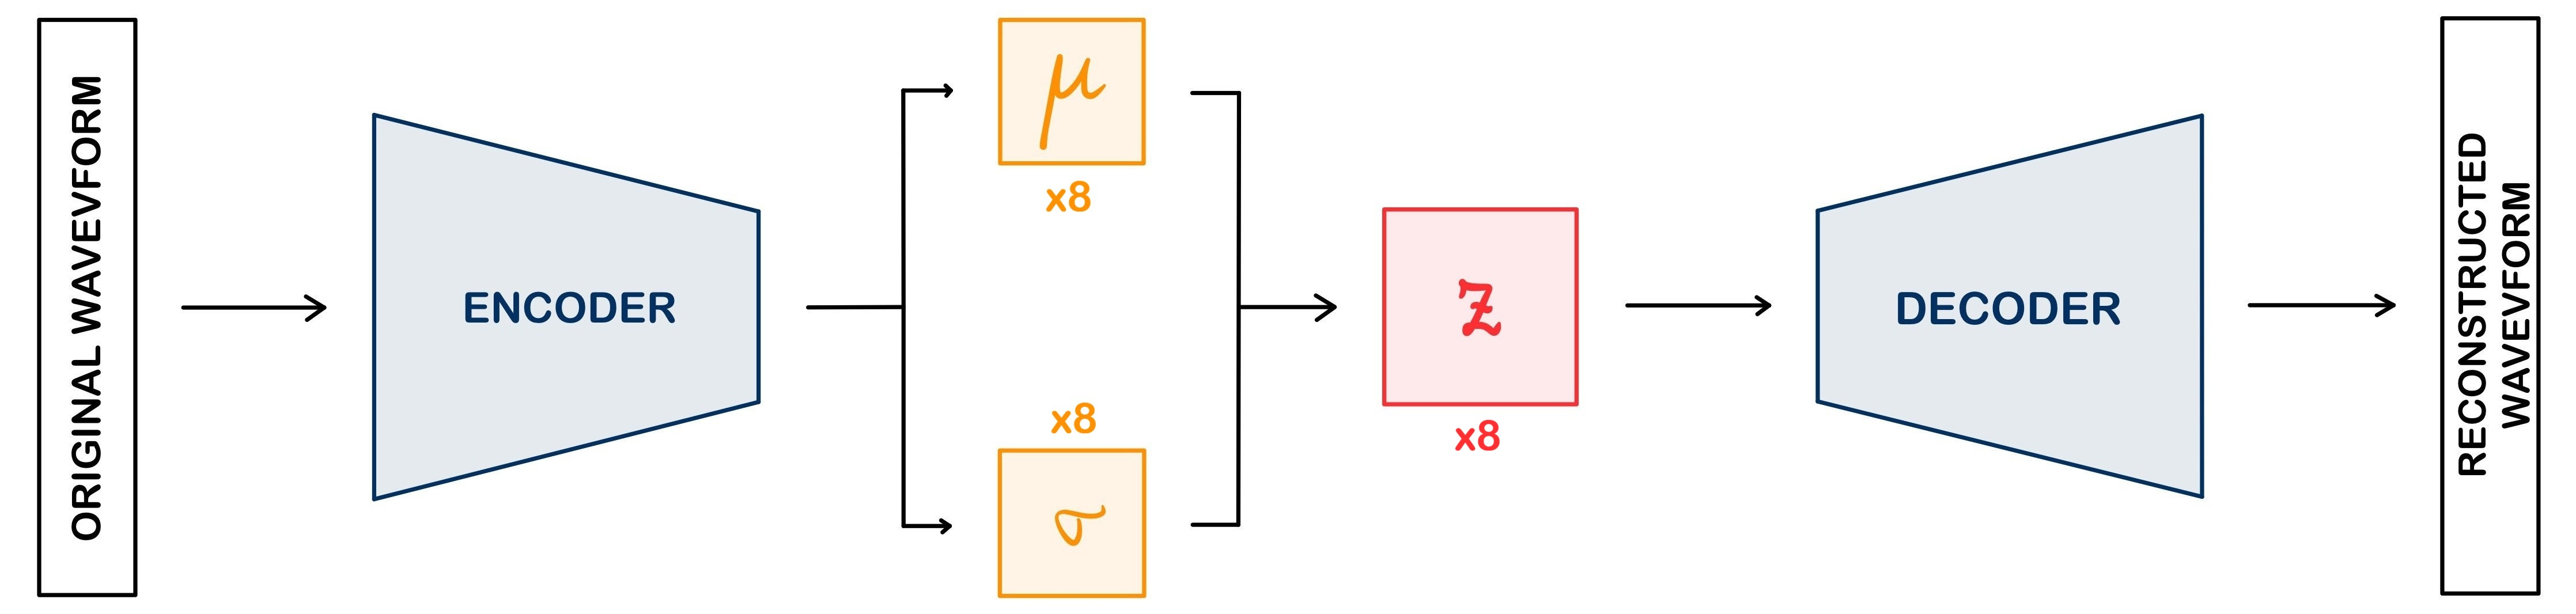
\includegraphics[width=\textwidth]{figures/schemaVAE.jpg}
    \caption{Schematic representation of the VAE architecture. The encoder network maps the input waveform to a latent space characterized by a mean and variance, from which a latent vector is sampled. The decoder reconstructs the waveform from this latent representation. The loss function combines reconstruction loss and KL divergence, weighted by the hyperparameter.}
    \label{fig:vae-architecture}
\end{figure}



\subsection{Training and testing}
\label{subsec:VAE-training}
The loss function that have been used is an \ac{ELBO}, i.e. the characteristic loss implemented in \ac{VAE} models, with some adjustments created for our specific work. The general formula is written in Eq. \ref{eq:ELBO} where it is visible that two terms enters in the loss computation: a reconstruction term and a regularisation one.
\begin{equation}
    \label{eq:ELBO}
    L = L_{\text{rec}} + \beta \cdot L_{\text{reg}}
\end{equation}

In the context of a \ac{VAE}, using a standard Mean Squared Error for the reconstruction loss would force the model to reproduce both the physically significant features of the waveform and the background stochastic noise, such as the random fluctuations preceding and following the main peaks. To overcome this limitation, the reconstruction term in the \ac{ELBO} function is modeled as the (\ac{NLL}) of a Gaussian distribution. Instead of assuming a fixed noise level, the \ac{VAE} dynamically learns a channel-specific variance, denoted as $\sigma_c^2$. This allows the model to weight the reconstruction error with respect to the expected noise level of each specific channel $c$.
Mathematically speaking, the squared error is divided by the learned variance $\sigma_c^2$, and a logarithmic penalty term ($\log \sigma_c^2$) is added. This second term is crucial to prevent a trivial solution: if the loss only consisted of the first term ($( x_{i,c,t} - \hat{x}_{i,c,t} )^2 / \sigma_c^2$), the optimization algorithm would simply predict an infinitely large noise value to drive the error to zero. The addition of the logarithmic penalty forces the model to find an optimal balance, preventing the overestimation of the underlying noise.
In this specific work, the two channels of the input tensor represent the charge and the current of the same physical signal. Since current is the time derivative of charge, these two quantities inherently possess fundamentally different scales and noise profiles. By learning a separate $\sigma_c^2$ for each channel, the \ac{NLL} acts as an automatic normalization mechanism, preventing the channel with the larger numerical magnitude or higher intrinsic variance from dominating the loss gradient. 
Finally, the individual losses of the channels must be summed, as expressed in Eq. \ref{eq:rec-loss}. From a probabilistic poin of view, this is equivalent to assuming independence of the noise between the charge and current measurements. Moreover, this sum is necessary to aggregate the array of channel-specific errors into a single scalar value, which is required by the framework to correctly perform the backpropagation algorithm.
\begin{equation}
    \label{eq:rec-loss}
    L_{\text{rec}} = \frac{1}{B} \sum_{i=1}^{B} \sum_{c=1}^{C} \left[ \frac{1}{2} \sum_{t=1}^{T} \left( \frac{\left( x_{i,c,t} - \hat{x}_{i,c,t} \right)^2}{\sigma_c^2} + \log \sigma_c^2 \right) \right]
\end{equation}

The second part of the loss expressed in Eq. \ref{eq:ELBO} concerns the organisation of the 8-dimension latent space and is based on \ac{KL} divergence. Firstly we define a \textit{prior} distribution, i.e. a standard Gaussian distribution $p(z) = \mathcal{N}(z; \mathbf{0}, \mathbf{I})$ with a zero mean vector and an identity covariance matrix. Secondly, seeing that the encoder network maps the original input waveform $x$ into a set of 8 Gaussian distributions, we can define the so-called \textit{posterior} distribution $q(z|x) = \mathcal{N}(z; \boldsymbol{\mu}_\phi(x), \text{diag}(\boldsymbol{\sigma}_\phi^2(x)))$, parameterized by the learned mean and variance vectors.
The \ac{KL} divergence is then computed to measure the statistical distance between the approximate \textit{posterior} and the \textit{prior}. This penalizes the model if the latent representations deviate significantly from a standard normal distribution. For a single latent dimension $j$, computed over a batch of size $B$, the analytical closed-form of the \ac{KL} divergence is given in Eq. \ref{eq:KL-loss}:
\begin{equation}
    \label{eq:KL-loss}
    D_{\text{KL},j} = \frac{1}{B} \sum_{i=1}^{B} \frac{1}{2} \left( \mu_{ij}^2 + \sigma_{ij}^2 - 1 - \log \sigma_{ij}^2 \right)
\end{equation}
In standard \ac{VAE} training, forcing strong regularization can lead to \textit{posterior collapse}: this occurs when the optimization algorithm drives the \ac{KL} divergence to zero by collapsing the posterior distribution to identically match the prior, effectively ignoring the input data and preventing the encoder from learning meaningful representations. 
To prevent this issue, a ``free bits'' (or \ac{KL} thresholding) strategy is implemented. Instead of forcing the divergence of every dimension to reach absolute zero, a minimum threshold $\lambda_{fb}$ is established. The total regularization loss $L_{\text{reg}}$ is computed by clamping the \ac{KL} divergence of each dimension to this lower bound before summing them, as defined in Eq. \ref{eq:KL-total} where $k$ is the number of dimensions in the latent space.
\begin{equation}
    \label{eq:KL-total}
    L_{\text{reg}} = \sum_{j=1}^{k} \max \left( \lambda_{fb}, \, D_{\text{KL},j} \right)
\end{equation}
By applying this maximum operator, the network is not forced to perfectly match the \textit{prior} distribution. If the divergence $D_{\text{KL},j}$ of a specific dimension drops below the chosen threshold $\lambda_{fb}$, the loss for that dimension remains constant at $\lambda_{fb}$. This means the encoder is allowed to retain a small amount of useful information (the \texttt{free bits}) to describe the waveform without being further penalized by the optimization process, effectively preventing the posterior collapse.

An additional tunable parameter $\beta$ balances the two contributions in the loss function: when $\beta < 1$ the reconstruction error weights more than the \ac{KL} thus the algorithm favours a truthful reconstruction, on the other hand if $\beta > 1$ the \ac{KL} becomes more important than the reconstruction. During the first part of the training a number $N_w$ of \textit{warm-up epochs} use a variable value of $\beta$ that is then settle to 1 as defined in Eq. \ref{eq:beta} where $n$ is the epoch number. This procedure is defined in order to let the algorithm learn appropriate weights for the reconstruction before trying to minimise the \ac{KL} divergence.
\begin{equation}
    \label{eq:beta}
    \beta(n) = \beta \cdot \min\left(1, \frac{n+1}{N_{\text{w}}}\right)
\end{equation}

The training and testing of the algorithm is done splitting the dataset in order to have the 90\% of the total available data for the training and validation sets and the 10\% of them for the test set.
Said 90\% is then splitted again, keeping the 90\% of it for the training set and the 10\% for the validation one. A number $N_w = 10$ of warm-up epochs have been used during the training phase of this algoritm. The number of dimensions in the latent space is $k = 8$.

The two following sections (\ref{subsec:VAE-features_extraction} and \ref{subsec:VAE-denoising}) will discuss two possible outcomes of the \ac{VAE} model, a feature extractor for a classification task and a denoising algorithm for current waveforms. However an initial verification of the robustness of its ability in the pure reconstruction task allows us to ensure the fact that if the reconstruction follows the waveform shape, the latent space is representative of the input as a consequence. Fig. \ref{fig:esempio-ricostruzione} and \ref{fig:esempio-losses} displays the reconstruction flow throught 100 epochs using $\beta=1$ and considering events within $3\sigma$ of the \ac{DEP} and \ac{FEP} as depicted in Fig. \ref{fig:sse_mse_cut}.

\begin{figure}[H]
    \centering
    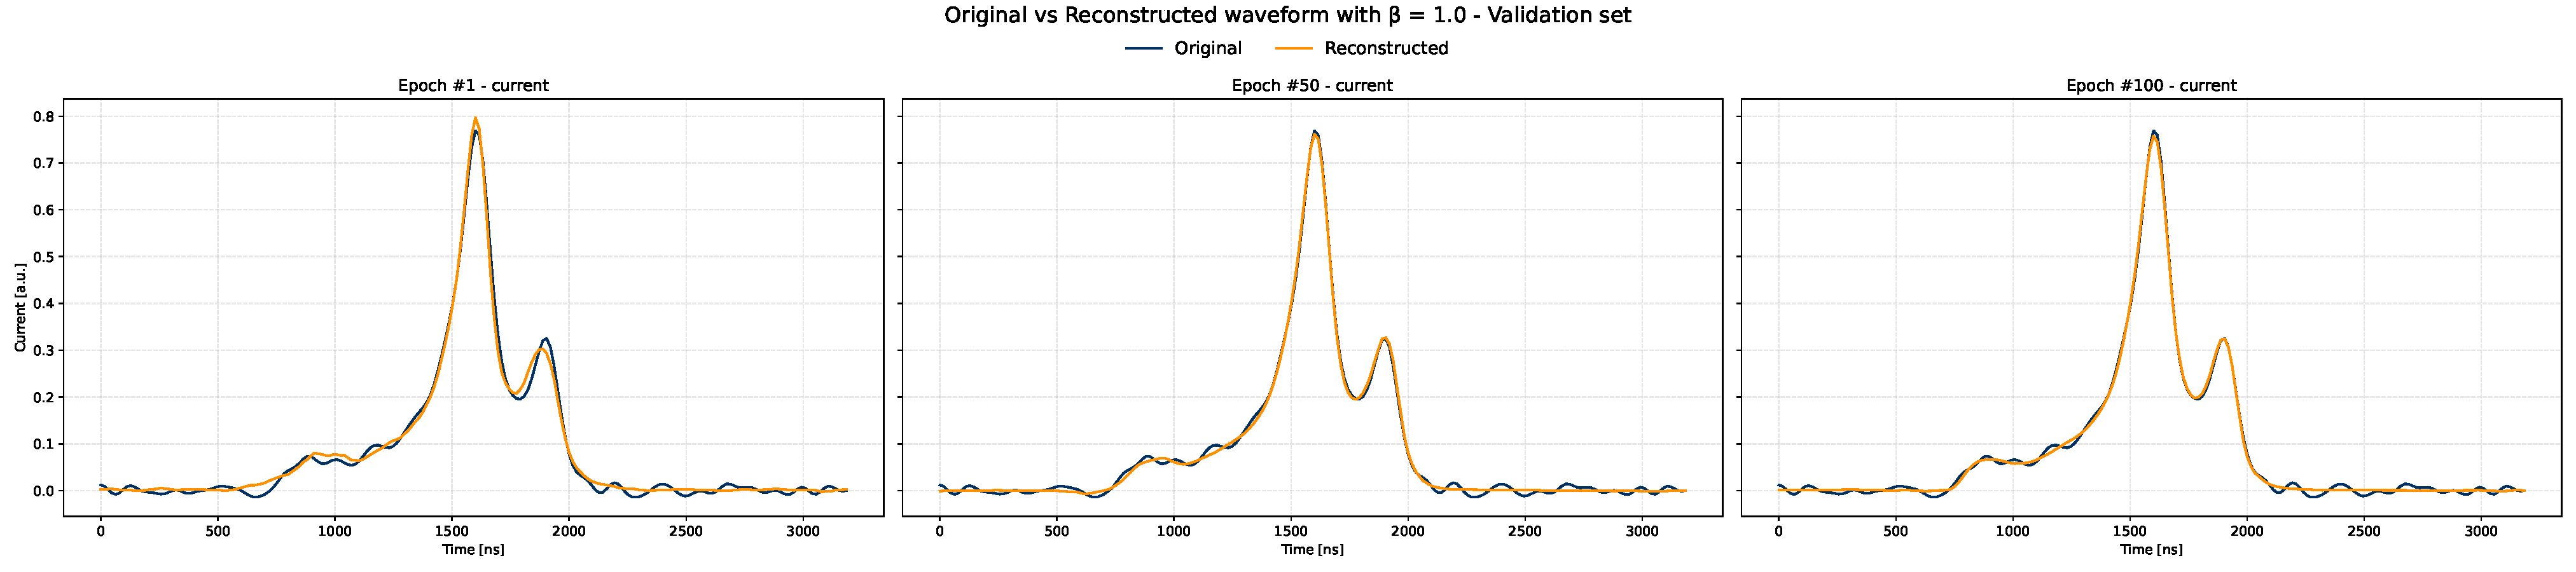
\includegraphics[width=\textwidth]{plots/VAEresults/beta1_sigma3_current_raw/validation_perEpoch_sigma3_current_raw_beta1.pdf}
    \caption{Decoder reconstrucion of validation set waveforms at epoch 1, 50 and 100}
    \label{fig:esempio-ricostruzione}
\end{figure}


\begin{figure}[H]
    \centering
    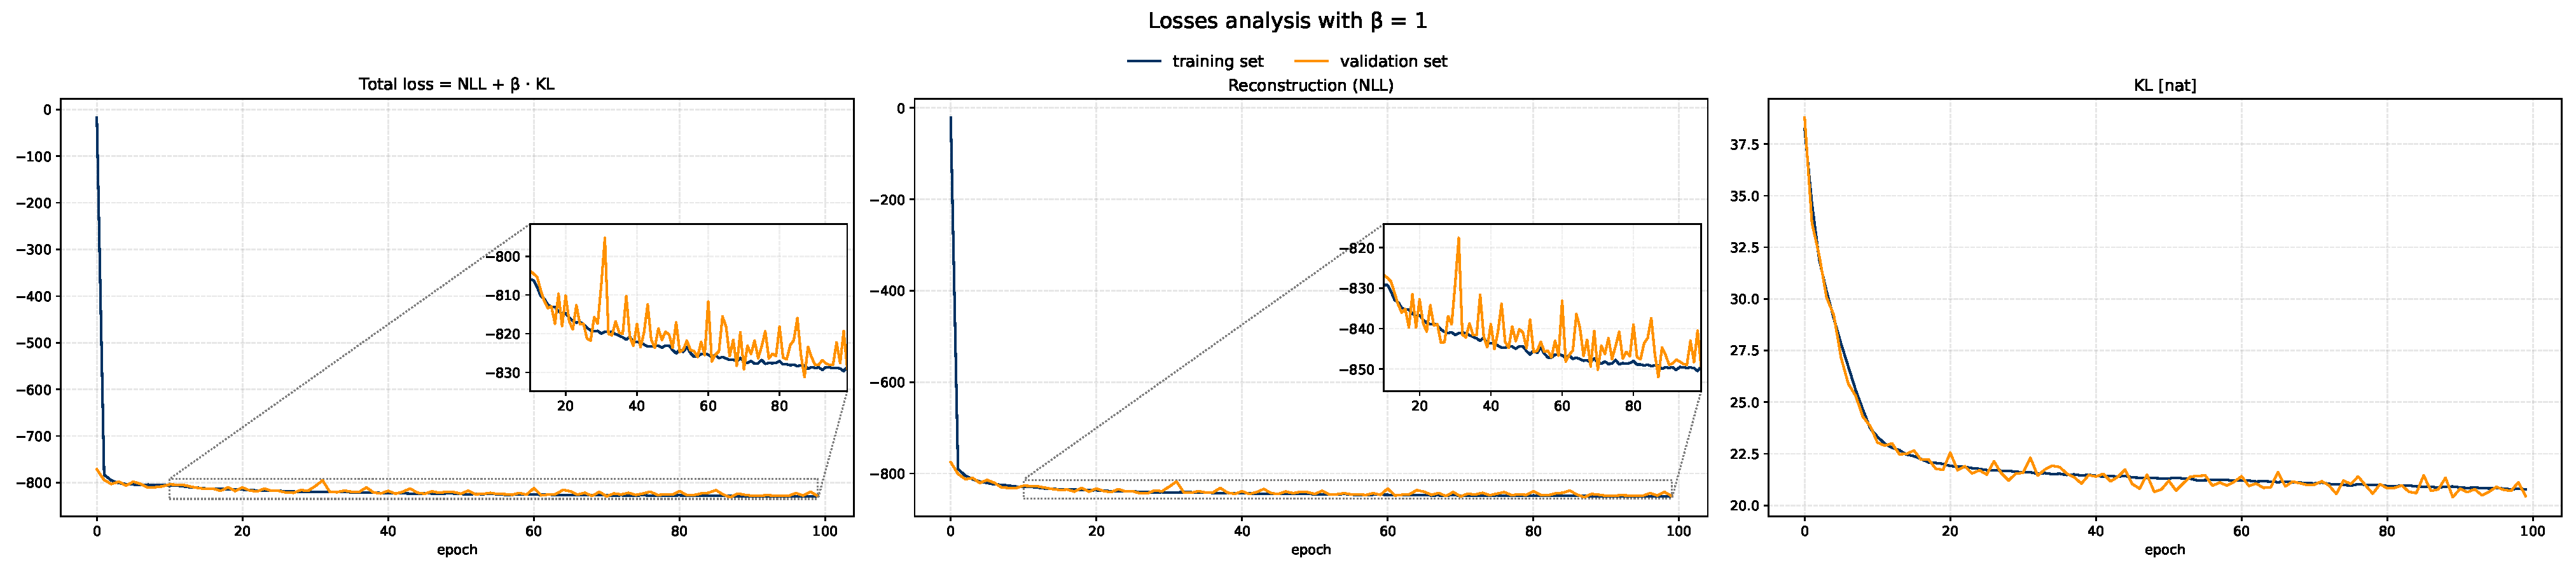
\includegraphics[width=\textwidth]{plots/VAEresults/beta1_sigma3_current_raw/train_valid_losses_sigma3_current_raw_beta1.pdf}
    \caption{Loss functions evolution through the training epochs. From the left to the right: total loss, reconstruction (\ac{NLL}) loss and \ac{KL} loss}
    \label{fig:esempio-losses}
\end{figure}



\subsection{\ac{VAE} as a feature extractor}
\label{subsec:VAE-features_extraction}
using beta1 and sigma3 

--- SSE SF with classifier = 59.95\% ---

--- MSE SF with classifier = 20.07\% ---

--- SSE SF with A/E = 59.10\% ---

--- MSE SF with A/E =  19.16\% ---

insomma uno schifo
\subsection{\ac{VAE} as a denoising algorithm}
\label{subsec:VAE-denoising}